\documentclass{beamer}
\input{../utils/preamble}
\createdgmtitle{8}
%--------------------------------------------------------------------------------
\begin{document}
%--------------------------------------------------------------------------------
\begin{frame}[noframenumbering,plain]
\titlepage
\end{frame}
%=======
\begin{frame}{Recap of Previous Lecture}
    \myfootnotewithlink{https://arxiv.org/abs/2403.18103}{Chan S. Tutorial on Diffusion Models for Imaging and Vision, 2024}
    \begin{block}{Forward Gaussian Diffusion Process}
        Let $\bx_0 = \bx \sim \pd(\bx)$, $\beta_t \ll 1$, $\alpha_t = 1 - \beta_t$ and $\bar{\alpha}_t = \prod_{s=1}^t \alpha_s$. 
        \begin{align*}
            \bx_t &= \sqrt{1 - \beta_t} \cdot \bx_{t - 1} + \sqrt{\beta_t} \cdot \bepsilon, \quad \text{where }\bepsilon \sim \cN(0, \bI); \\
            \bx_t &= \sqrt{\bar{\alpha}_t} \cdot \bx_{0} + \sqrt{1 - \bar{\alpha}_t} \cdot \bepsilon, \quad \text{where } \bepsilon \sim \cN(0, \bI).
        \end{align*}
        \vspace{-0.6cm}
        \begin{align*}
            q(\bx_t | \bx_{t-1}) &= \cN(\sqrt{1 - \beta_t} \cdot \bx_{t-1}, \beta_t \cdot \bI); \\
            q(\bx_t | \bx_0) &= \cN(\sqrt{\bar{\alpha}_t} \cdot \bx_0, (1 - \bar{\alpha}_t) \cdot \bI).
        \end{align*}
        \vspace{-0.6cm}
    \end{block}
    \begin{figure}
        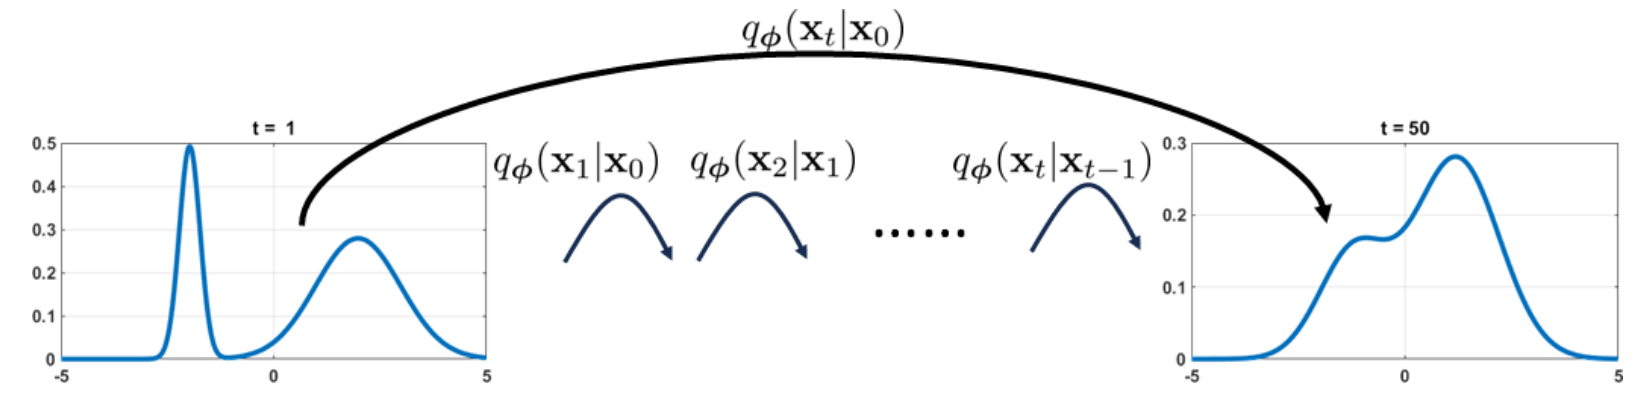
\includegraphics[width=0.8\linewidth]{figs/conditional_diffusion}
    \end{figure}
\end{frame}
%=======
\begin{frame}{Recap of Previous Lecture}
    \myfootnotewithlink{https://ayandas.me/blog-tut/2021/12/04/diffusion-prob-models.html}{Das A. An Introduction to Diffusion Probabilistic Models, blog post, 2021}
    \textbf{Diffusion} describes the process where particles migrate from regions of high density to regions of low density.
    \vspace{-0.2cm}
    \begin{figure}
        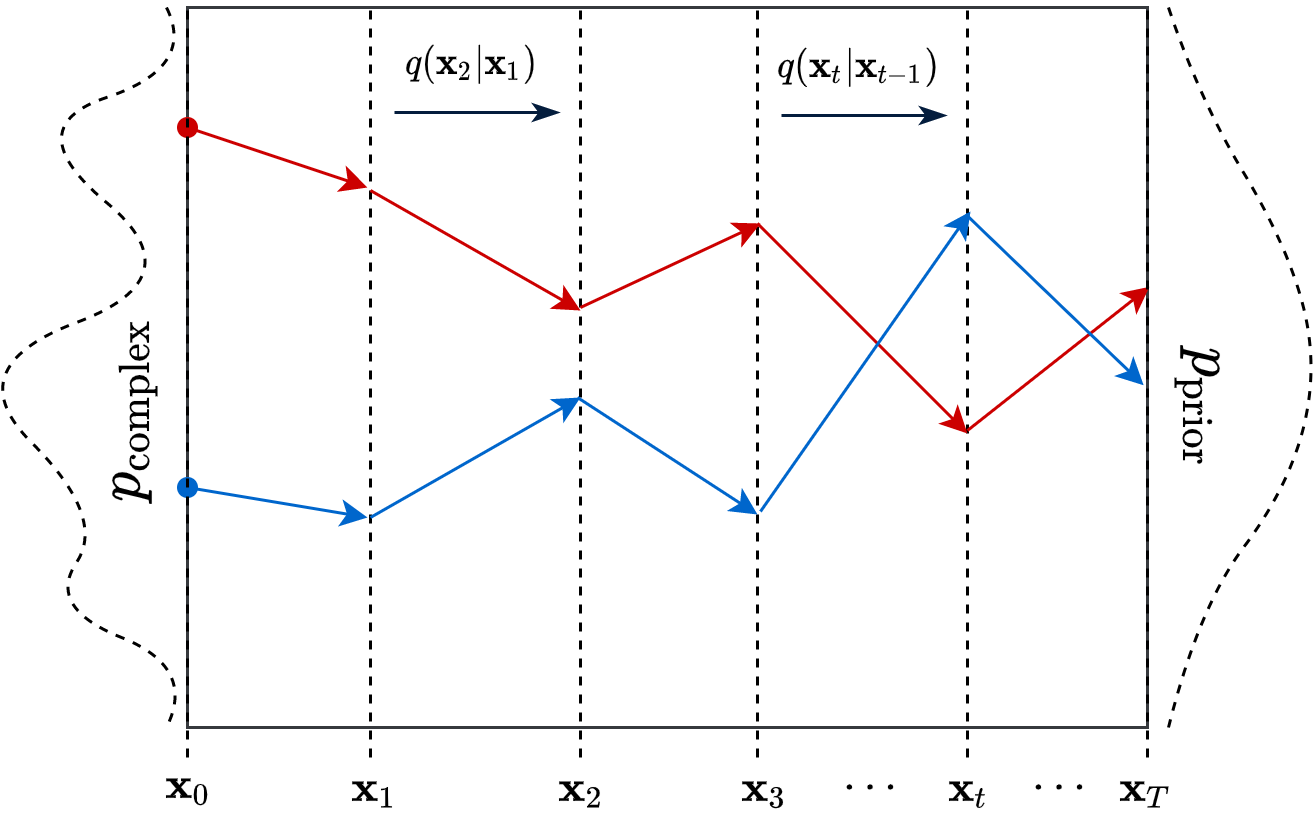
\includegraphics[width=0.5\linewidth]{figs/diffusion_over_time}
    \end{figure}
    \vspace{-0.6cm}
    \begin{enumerate}
        \item $\bx_0 = \bx \sim \pd(\bx)$;
        \item $\bx_t = \sqrt{1 - \beta_t} \cdot \bx_{t - 1} + \sqrt{\beta_t} \cdot \bepsilon$, with $\bepsilon \sim \cN(0, \bI)$, $t \geq 1$;
        \item $\bx_T \sim p_{\infty}(\bx) = \cN(0, \bI)$, for $T \gg 1$.
    \end{enumerate}
    If we can invert this process, we would have a way to sample $\bx \sim \pd(\bx)$ using noise samples, i.e. $p_{\infty}(\bx) = \cN(0, \bI)$. \\ 
    Hence, our objective becomes to reverse this process.
\end{frame}
%=======
\begin{frame}{Recap of Previous Lecture}
    \myfootnotewithlink{https://lilianweng.github.io/posts/2021-07-11-diffusion-models/}{Weng L. What are Diffusion Models?, blog post, 2021}
    \vspace{-0.3cm}
    \begin{figure}
        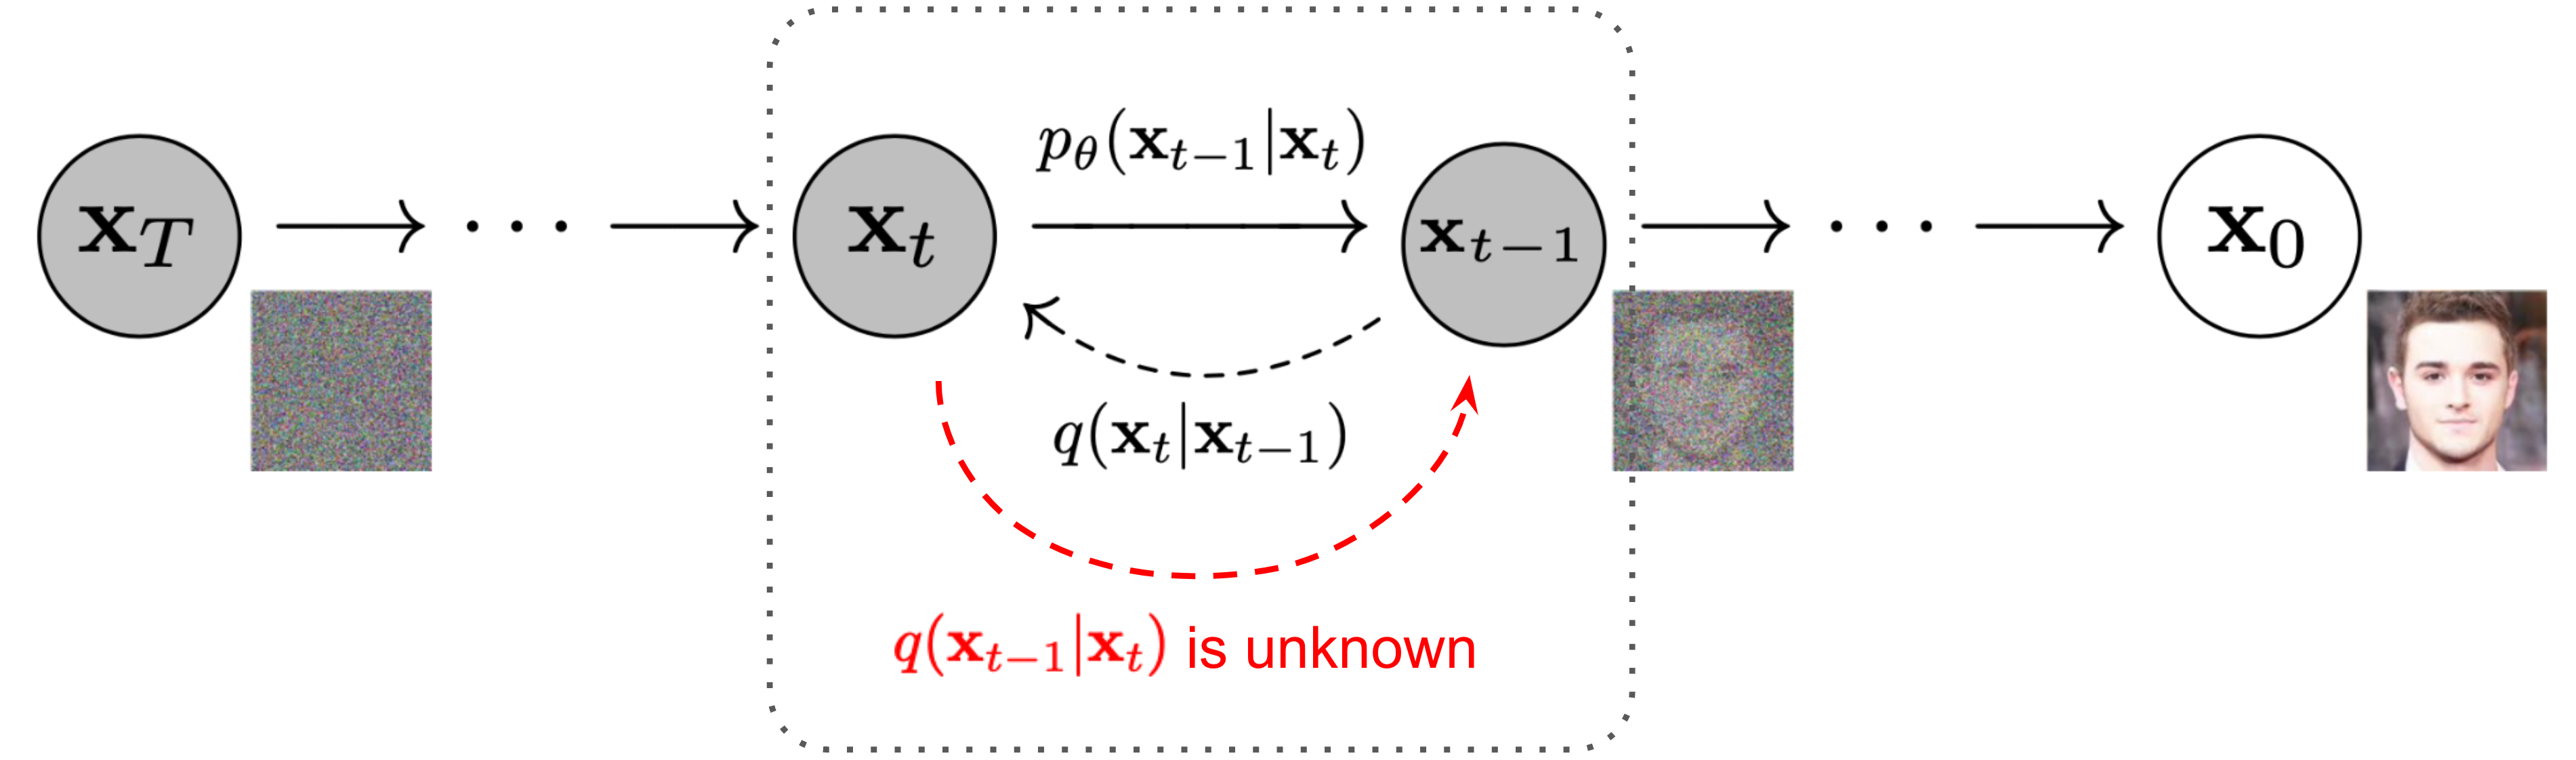
\includegraphics[width=0.8\linewidth]{figs/DDPM}
    \end{figure}
    \vspace{-0.5cm}
    \begin{block}{Reverse Process (Ancestral Sampling)}
        \vspace{-0.5cm}
        {\small
        \[
            q(\bx_{t-1}|\bx_{t}) = \frac{q(\bx_{t}|\bx_{t-1}) {\color{violet}q(\bx_{t-1})}}{{\color{violet}q(\bx_{t})}} \approx \pt(\bx_{t - 1} | \bx_t) = \cN \left(\bmu_{\btheta, t}(\bx_t), \bsigma_{\btheta, t}^2(\bx_t)\right)
        \]}
        {\color{gray}The Feller theorem guarantees this approximation is valid.}
    \end{block}
    \begin{minipage}{0.5\linewidth}
        \begin{block}{Forward Process}
            \begin{enumerate}
                \item $\bx_0 = \bx \sim \pd(\bx)$;
                \item $\bx_t = \sqrt{1 - \beta_t} \cdot \bx_{t - 1} + \sqrt{\beta_t} \cdot \bepsilon$;
                \item $\bx_T \sim p_{\infty}(\bx) = \cN(0, \bI)$.
            \end{enumerate}
        \end{block}
    \end{minipage}%
    \begin{minipage}{0.55\linewidth}
        \begin{block}{Reverse Process}
            \begin{enumerate}
                \item $\bx_T \sim p_{\infty}(\bx) = \cN(0, \bI)$;
                \item $\bx_{t - 1} = \bsigma_{\btheta, t}(\bx_t) \cdot \bepsilon + \bmu_{\btheta, t}(\bx_t)$;
                \item $\bx_0 = \bx \sim \pd(\bx)$;
            \end{enumerate}
        \end{block}
    \end{minipage}
\end{frame}
%=======
\begin{frame}{Outline}
    \tableofcontents
\end{frame}
%=======
\section{Reparametrization}
%=======
\begin{frame}{Reparametrization of DDPM}
    \myfootnotewithlink{https://arxiv.org/abs/2006.11239}{Ho J. Denoising Diffusion Probabilistic Models, 2020}
    \[
        \cL_t = \bbE_{q(\bx_t | \bx_0)} \left[\frac{1}{2\tilde{\beta}_t} \bigl\| \tilde{\bmu}_t(\bx_t, \bx_0) - \bmu_{\btheta, t}(\bx_t) \bigr\|^2  \right]
    \]
    \[
        \tilde{\bmu}_t(\bx_t, \bx_0) = \frac{\sqrt{\alpha_t}(1 - \bar{\alpha}_{t-1})}{1 - \bar{\alpha}_t} \cdot \bx_t + \frac{\sqrt{\bar{\alpha}_{t-1}}(1 - \alpha_t)}{1 - \bar{\alpha}_t} \cdot {\color{olive} \bx_0}
    \]
    \eqpause
    \vspace{-0.2cm}
    \[
        \bx_t = \sqrt{\bar{\alpha}_t} \cdot \bx_0 + \sqrt{1 - \bar{\alpha}_t} \cdot \bepsilon \quad \nextonslide{\Rightarrow \quad {\color{olive} \bx_0} = \frac{\bx_t -  \sqrt{1 - \bar{\alpha}_t} \cdot \bepsilon}{\sqrt{\bar{\alpha}_t}}}
    \]
    \eqpause
    \vspace{-0.3cm}
    \begin{itemize}
        \item There is a linear relationship between $\bepsilon$, $\bx_t$, and $\bx_0$.
        \item Let's try to rewrite this mean using only $\bx_t$ and $\bepsilon$.
    \end{itemize}
    \eqpause
    \vspace{-0.2cm}
    \begin{align*}
        \tilde{\bmu}_t(\bx_t, \bepsilon) &= \frac{\sqrt{\alpha_t}(1 - \bar{\alpha}_{t-1})}{1 - \bar{\alpha}_t} \cdot \bx_t + \frac{\sqrt{\bar{\alpha}_{t-1}}(1 - \alpha_t)}{1 - \bar{\alpha}_t} \cdot {\color{olive} \left(\frac{\bx_t -  \sqrt{1 - \bar{\alpha}_t} \cdot \bepsilon}{\sqrt{\bar{\alpha}_t}}\right)} \\
        \nextonslide{&= \frac{1}{\sqrt{\alpha_t}} \cdot \bx_t - \frac{1 - \alpha_t}{\sqrt{\alpha_t (1 - \bar{\alpha}_t)}} \cdot \bepsilon}
    \end{align*}
\end{frame}
%=======
\begin{frame}{Reparametrization of DDPM}
    \myfootnotewithlink{https://arxiv.org/abs/2006.11239}{Ho J. Denoising Diffusion Probabilistic Models, 2020}
    \[
        \cL_t = \bbE_{\color{violet}q(\bx_t | \bx_0)} \left[ {\color{olive}\frac{1}{2\tilde{\beta}_t}} \bigl\| \tilde{\bmu}_t(\bx_t, \bx_0) - \bmu_{\btheta, t}(\bx_t) \bigr\|^2  \right]
    \]
    \vspace{-0.3cm}
    \begin{block}{Reparametrization}
        \vspace{-0.7cm}
        \begin{align*}
            \tilde{\bmu}_t(\bx_t, \bx_0) &= \frac{1}{\sqrt{\alpha_t}} \cdot \bx_t - \frac{1 - \alpha_t}{\sqrt{\alpha_t (1 - \bar{\alpha}_t)}} \cdot \bepsilon \\
            \nextonslide{\bmu_{\btheta, t}(\bx_t) &= \frac{1}{\sqrt{\alpha_t}} \cdot \bx_t - {\color{teal}\frac{1 - \alpha_t}{\sqrt{\alpha_t (1 - \bar{\alpha}_t)}}} \cdot \bepsilon_{\btheta, t}(\bx_t)}
        \end{align*}
        \vspace{-0.7cm}
    \end{block}
    \eqpause
    \vspace{-0.5cm}
    \begin{align*}
        \cL_t &=  \bbE_{\color{violet} \bepsilon \sim \cN(0, \bI)} \left[ \frac{{\color{teal}(1 - \alpha_t)^2}}{{\color{olive}2\tilde{\beta}_t} {\color{teal} \alpha_t (1 - \bar{\alpha}_t)}} \bigl\| \bepsilon - \bepsilon_{\btheta, t}({\color{violet}\bx_t}) \bigr\|^2 \right] \\
        \nextonslide{& =  \bbE_{\color{violet}\bepsilon \sim \cN(0, \bI)} \left[ \frac{(1 - \alpha_t)^2}{2\tilde{\beta}_t \alpha_t (1 - \bar{\alpha}_t)} \Bigl\| \bepsilon - \bepsilon_{\btheta, t}\bigl( {\color{violet}\sqrt{\bar{\alpha}_t} \bx_0 + \sqrt{1 - \bar{\alpha}_t} \bepsilon}\bigr) \Bigr\|^2 \right]}
    \end{align*}
    \eqpause
    At every step of the reverse process, we attempt to predict the noise~$\bepsilon$ that was used in the forward diffusion process!
\end{frame}
%=======
\begin{frame}{Reparametrization of DDPM}
    \myfootnotewithlink{https://arxiv.org/abs/2006.11239}{Ho J. Denoising Diffusion Probabilistic Models, 2020}
    \begin{multline*}
        \cL_{\bphi, \btheta}(\bx) =  {\color{olive}\bbE_{q(\bx_1 | \bx_0)} \log \pt(\bx_0 | \bx_1)} - {\color{violet}\KL\bigl(q(\bx_T | \bx_0) \| p(\bx_T)\bigr)} - \\
        - \sum_{t=2}^T \underbrace{ \bbE_{q(\bx_t | \bx_0)} \KL \bigl(q(\bx_{t-1} | \bx_t, \bx_0) \| \pt(\bx_{t-1} | \bx_t)\bigr)}_{\cL_t}
    \end{multline*}
    \eqpause
    \vspace{-0.3cm}
    \[
        \cL_t  = \bbE_{\bepsilon \sim \cN(0, \bI)} \left[ \frac{(1 - \alpha_t)^2}{2\tilde{\beta}_t \alpha_t (1 - \bar{\alpha}_t)} \Bigl\| \bepsilon - \bepsilon_{\btheta, t}\bigl( \sqrt{\bar{\alpha}_t} \bx_0 + \sqrt{1 - \bar{\alpha}_t} \bepsilon\bigr) \Bigr\|^2 \right]
    \]
    \eqpause
    Let's drop the scaling coefficient.
    \begin{block}{Simplified Objective}
        \vspace{-0.3cm}
        \[
             \cL_{\text{simple}} = \bbE_{t \sim U\{2, T\}} \bbE_{\bepsilon \sim \cN(0, \bI)} \Bigl\| \bepsilon - \bepsilon_{\btheta, t}\bigl( \sqrt{\bar{\alpha}_t} \cdot \bx_0 + \sqrt{1 - \bar{\alpha}_t} \cdot \bepsilon\bigr) \Bigr\|^2 
        \]
    \end{block}
\end{frame}
%=======
\section{Denoising Diffusion Probabilistic Model (DDPM)}
%=======
\begin{frame}{Generative Models Taxonomy}
	\renderTaxonomy{ddpm}
\end{frame}
%=======
\begin{frame}{Denoising Diffusion Probabilistic Model (DDPM)}
    \myfootnotewithlink{https://arxiv.org/abs/2006.11239}{Ho J. Denoising Diffusion Probabilistic Models, 2020}
    \begin{block}{DDPM is a VAE Model}
        \begin{itemize}
            \item The encoder is a fixed Gaussian Markov chain $q(\bx_1, \dots, \bx_T | \bx_0)$.
            \item The latent variable is hierarchical (at each step, its dimension equals the input's).
            \item The decoder is a simple Gaussian model $\pt(\bx_0 | \bx_1)$.
            \item The prior distribution is given by a parametric Gaussian Markov chain $\pt(\bx_{t-1} | \bx_t)$.
        \end{itemize}
    \end{block}
    \eqpause
    \begin{minipage}{0.5\linewidth}
        \begin{block}{Forward Process}
            \begin{enumerate}
                \item $\bx_0 = \bx \sim \pd(\bx)$;
                \item $\bx_t = \sqrt{1 - \beta_t} \cdot \bx_{t - 1} + \sqrt{\beta_t} \cdot \bepsilon$;
                \item $\bx_T \sim p_{\infty}(\bx) = \cN(0, \bI)$.
            \end{enumerate}
        \end{block}
    \end{minipage}%
    \eqpause
    \begin{minipage}{0.55\linewidth}
        \begin{block}{Reverse Process}
            \begin{enumerate}
                \item $\bx_T \sim p_{\infty}(\bx) = \cN(0, \bI)$;
                \item $\bx_{t - 1} = \bsigma_{\btheta, t}(\bx_t) \cdot \bepsilon + \bmu_{\btheta, t}(\bx_t)$;
                \item $\bx_0 = \bx \sim \pd(\bx)$;
            \end{enumerate}
        \end{block}
    \end{minipage}
\end{frame}
%=======
\begin{frame}{Denoising Diffusion Probabilistic Model (DDPM)}
    \myfootnotewithlink{https://arxiv.org/abs/2006.11239}{Ho J. Denoising Diffusion Probabilistic Models, 2020}
    \begin{block}{Training}
        \begin{enumerate}
            \item Obtain a sample $\bx_0 \sim \pd(\bx)$.
            \item Sample time index $t \sim U\{1, T\}$ and noise $\bepsilon \sim \cN(0, \bI)$.
            \item Generate noisy image $\bx_t = \sqrt{\bar{\alpha}_t} \cdot \bx_0 + \sqrt{1 - \bar{\alpha}_t} \cdot \bepsilon$.
            \item Compute the loss $ \cL_{\text{simple}} = \| \bepsilon - \bepsilon_{\btheta, t}(\bx_t) \|^2 $.
        \end{enumerate}
    \end{block}
    \eqpause
    \begin{block}{Sampling (Ancestral Sampling)}
        \begin{enumerate}
            \item Sample $\bx_T \sim \cN(0, \bI)$.
            \item Compute the mean of $\pt(\bx_{t-1} | \bx_t) = \cN(\bmu_{\btheta, t}(\bx_t), \tilde{\beta}_t \cdot \bI)$:
            \[
                \bmu_{\btheta, t}(\bx_t) = \frac{1}{\sqrt{\alpha_t}} \cdot \bx_t - \frac{1 - \alpha_t}{\sqrt{\alpha_t (1 - \bar{\alpha}_t)}} \cdot \bepsilon_{\btheta, t}(\bx_t)
            \]
            \vspace{-0.3cm}
            \item Denoise: $\bx_{t - 1} = \bmu_{\btheta, t}(\bx_t) +  \sqrt{\tilde{\beta}_t} \cdot \bepsilon$, $\bepsilon \sim \cN(0, \bI)$.
        \end{enumerate}
    \end{block}
\end{frame}
%=======
\begin{frame}{Denoising Diffusion Probabilistic Model (DDPM)}
    \myfootnotewithlink{https://arxiv.org/abs/2006.11239}{Ho J. Denoising Diffusion Probabilistic Models, 2020}
    \begin{block}{Samples}
        \begin{figure}
            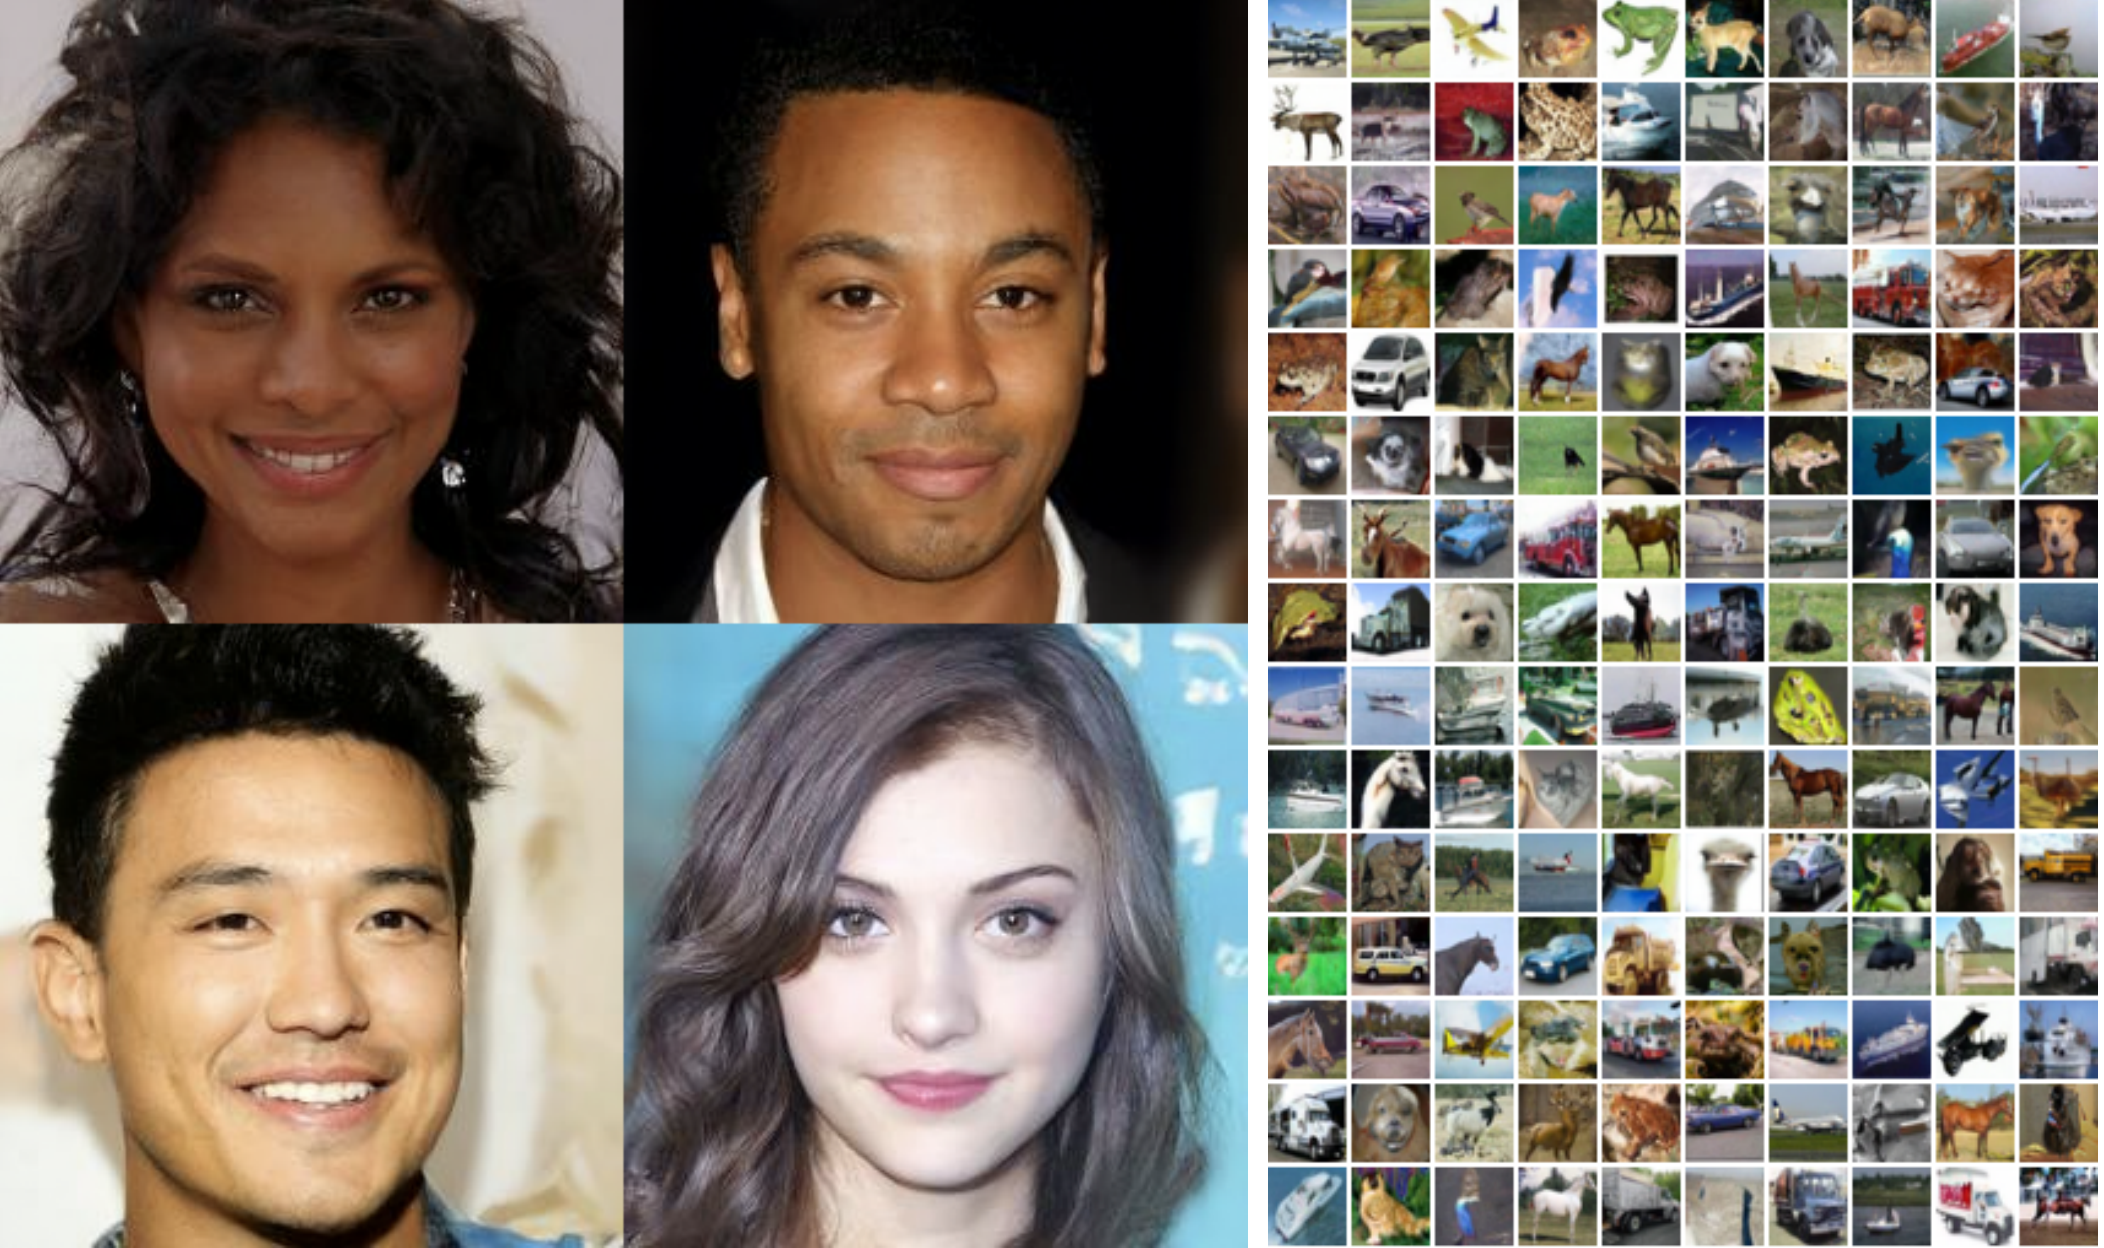
\includegraphics[width=\linewidth]{figs/ddpm_samples}
        \end{figure}
    \end{block}
\end{frame}
%=======
\begin{frame}{Summary}
    \begin{itemize}
        \item At each step, DDPM predicts the noise that was injected in the forward process. 
        \vfill
        \item DDPM is a VAE model that tries to invert the forward diffusion process via variational inference. 
        \vfill
        \item DDPMs are quite slow, since the model must be applied $T$ times for sampling.
    \end{itemize}
\end{frame}
%=======
\end{document}